\UseRawInputEncoding
% !TEX TS-program = pdflatex
% !TEX encoding = UTF-8 Unicode


\documentclass[11pt]{article} % use larger type; default would be 10pt

%\usepackage[utf8]{inputenc} % set input encoding (not needed with XeLaTeX)


%%% PAGE DIMENSIONS
\usepackage{geometry}
\geometry{a4paper} 

\usepackage{graphicx} 

% \usepackage[parfill]{parskip} % Activate to begin paragraphs with an empty line rather than an indent

%%% PACKAGES

\usepackage{setspace}
\usepackage{listings}
\usepackage{hyperref}
\hypersetup{
    colorlinks=true,
    linkcolor=blue,
    filecolor=magenta,      
    urlcolor=cyan,
}

\usepackage{color}
\definecolor{dkgreen}{rgb}{0,0.6,0}
\definecolor{gray}{rgb}{0.5,0.5,0.5}
\definecolor{mauve}{rgb}{0.58,0,0.82}

\lstset{frame=L,
  language=Python,
  aboveskip=3mm,
  belowskip=3mm,
  showstringspaces=false,
  columns=flexible,
  basicstyle={\small\ttfamily},
  numbers=none,
  numberstyle=\tiny\color{gray},
  keywordstyle=\color{blue},
  commentstyle=\color{dkgreen},
  stringstyle=\color{mauve},
  breaklines=true,
  breakatwhitespace=true,
  tabsize=3
}
\usepackage{booktabs} % for much better looking tables
\usepackage{array} % for better arrays (eg matrices) in maths
\usepackage{paralist} % very flexible & customisable lists (eg. enumerate/itemize, etc.)
\usepackage{verbatim} % adds environment for commenting out blocks of text & for better verbatim
\usepackage{subfig} % make it possible to include more than one captioned figure/table in a single float
% These packages are all incorporated in the memoir class to one degree or another...

%%% HEADERS & FOOTERS
\usepackage{fancyhdr} % This should be set AFTER setting up the page geometry
\pagestyle{fancy} % options: empty , plain , fancy
\renewcommand{\headrulewidth}{0pt} % customise the layout...
\lhead{}\chead{}\rhead{}
\lfoot{}\cfoot{\thepage}\rfoot{}

%%% SECTION TITLE APPEARANCE
\usepackage{sectsty}
\allsectionsfont{\sffamily\mdseries\upshape} % (See the fntguide.pdf for font help)
% (This matches ConTeXt defaults)

%%% ToC (table of contents) APPEARANCE
\usepackage[nottoc,notlof,notlot]{tocbibind} % Put the bibliography in the ToC
\usepackage[titles,subfigure]{tocloft} % Alter the style of the Table of Contents
\renewcommand{\cftsecfont}{\rmfamily\mdseries\upshape}
\renewcommand{\cftsecpagefont}{\rmfamily\mdseries\upshape} % No bold!

%%% END Article customizations

%%% The "real" document content comes below...

\title{Wine Reviews Data Analasys}
\author{Anja Miletic}
%\date{} % Activate to display a given date or no date (if empty),
         % otherwise the current date is printed 

\begin{document}
\pagenumbering{gobble}
\maketitle
\newpage

\doublespacing
\tableofcontents
\singlespacing
\newpage

\pagenumbering{arabic}

\section{Uvod}
Podaci su skinuti na linku \url{https://www.kaggle.com/zynicide/wine-reviews}. Podaci predstavljaju recenzije razlicitih vrsta vina
koje su postavljali korsnici sajta WineEnthusiast.

\section{Analiza i pretprocesiranje podataka}
Podatke prvo otvaramo u programu KNIME preko cvora CSV Reader. Medjutim, podaci se ne mogu odmah otvoriti.
Analizom gresaka koje ispisuje program ustanovljena su dva problema; u nekim kolonama postoji znak \# koji 
KNIME gleda kao pocetak komentara, i u koloni description se javlja znak za novi red \textbackslash n. Iskljucujemo opcije 
za komentare i rucno brisemo nove redove unutar kolone description. Sada mozemo otvoriti datoteku.
\footnote{zbog tipa tekstualnih podataka enkodiranje je promenjeno u utf-8}

Tabela sadrzi oko 150 hiljada redova i 10 atributa (kolona). Opisi kolona su dati u tabeli 1.
\newline\newline
\begin{tabular}{|l|l|}
\hline
country & drzava iz koje je vino \\
\hline
description & tekst recenzije \\
\hline
designation & vinograd unutar vinarije iz kojeg je grozdje od kojeg je napravljeno vino \\
\hline
points & broj poena (od 100) sa kojima je ocenjeno vino \\
\hline
price & cena za flasu vina u dolarima \\
\hline
province & provincija ili savezna drzava iz koje je vino \\
\hline
region\_1 & regija provincije ili savezne drzave gde raste loza \\
\hline
region\_2 & ukoliko postoji, preciznija lokacija gde raste loza \\
\hline
variety & vrsta grozdja koje se koristilo \\
\hline
winery & ime vinarije koja je napravila vino \\
\hline
\end{tabular}

\subsection{Analiza podataka}

Koristimo Python kod da izlistamo osnovne informacije o podacima.
\begin{lstlisting}
import pandas

import pandas as pd 
import matplotlib.pyplot as plt 
import numpy as np 

def main():
	df = pd.read_csv("./winemag-data_first150k.csv")

	df = df.drop(labels=['Unnamed: 0'], axis=1)

	print(df.head())
	print(df.count())
	print(df.dtypes)
	
	print(df.describe())
	
\end{lstlisting}
rezultat izvrsavanja:
\begin{lstlisting}
  country                                        description
0      US  This tremendous 100% varietal wine hails from ...
1   Spain  Ripe aromas of fig, blackberry and cassis are ... 
2      US  Mac Watson honors the memory of a wine once ma...
3      US  This spent 20 months in 30% new French oak, an...
4  France  This is the top wine from La Bégude, named aft...

                           designation           ...                      region_2 
                     Martha's Vineyard           ...                          Napa 
 Carodorum Seleccion Especial Reserva           ...                           NaN 
         Special Selected Late Harvest           ...                        Sonoma 
                               Reserve           ...             Willamette Valley 
                            La Brûlade           ...                           NaN 

            variety                   winery
 Cabernet Sauvignon                    Heitz
      Tinta de Toro  Bodega Carmen Rodríguez
    Sauvignon Blanc                 Macauley
         Pinot Noir                    Ponzi
 Provence red blend     Domaine de la Bégude

#broj ne null vrednosti 
country        150925
description    150930
designation    105192
points         150930
price          137235
province       150925
region_1       125870
region_2        60953
variety        150930
winery         150930

#tipovi atributa
country         object
description     object
designation     object
points           int64
price          float64
province        object
region_1        object
region_2        object
variety         object
winery          object

#statisticki podaci numerickih atributa
              points          price
count  150930.000000  137235.000000
mean       87.888418      33.131482
std         3.222392      36.322536
min        80.000000       4.000000
25%        86.000000      16.000000
50%        88.000000      24.000000
75%        90.000000      40.000000
max       100.000000    2300.000000
\end{lstlisting}

Primecujemo da 4 atributa nemaju nijednu null vrednost (description, points, variety, winery). Takodje,
svi poeni su u intervalu 80-100, sa prosecnom ocenom od oko 87 poena. Sto se tice cene flase vina, iako je 
najveca vrednost cak 2300 dolara, vidimo da treci kvantil ima vrednost od 40\$, odnosno da je vecina vrednosti
do 50\$. U nasoj analizi zanemaricemo vrednosti preko 50\$.\newline 
Sada cemo da grupisemo vrednosti atributa i izlistamo ih.
\begin{lstlisting}
for col in df.columns:
	print("count values in column " + col)
	print(df[col].value_counts(dropna = False))
\end{lstlisting}
Ispis iz konzole:
\begin{lstlisting}
count values in column country
US                        62397
Italy                     23478
France                    21098
Spain                      8268
Chile                      5816
..
Name: country, dtype: int64

count values in column description
Powerful in Zinny character, this blend of Dry ..                                                                                    6
This could work as a rich wine, because there..                                                                                    6
Barrel sample. A rounded wine, its tannins ..                                                                                    6
..
Name: description, Length: 97821, dtype: int64

count values in column designation
NaN                                          45738
Reserve                                       2752
Reserva                                       1810
Estate                                        1571
Barrel sample                                 1326
..
Name: designation, Length: 30620, dtype: int64

count values in column province
California                                44508
Washington                                 9750
Tuscany                                    7281
Bordeaux                                   6111
Northern Spain                             4892
..
\end{lstlisting}
Najvise vina je iz Amerike, tako da su najcesce dve vrednosti u koloni province takodje iz Amerike.\newline
Primetimo da u koloni description u kojoj ne bi trebalo da postoje identicne vrednosti, postoji recenzija koja se 
pojavljuje cak 6 puta. Zakljucujemo da postoje duplikati vrednosti. Funkcijom \lstinline{DataFrame.drop_duplicates()}
brisemo takve redove, ostavljajuci jedan. Zatim opet brojimo ne-null vrednosti:

\begin{lstlisting}
country        97848
description    97851
designation    67953
points         97851
price          89131
province       97848
region_1       81919
region_2       39491
variety        97851
winery         97851
\end{lstlisting}

Dakle oko trecina podataka su bili duplikati. Sada imamo oko 100 hiljada redova.\newline
Kolone cena i poeni sadrze numericke vrednosti. Koristimo \lstinline{hexbin} koji predstavlja 
dvodimenzionalni histogram sa heksagonalnim celijama da vidimo distribuciju vrednosti ove dve
kolone. 
Takodje nam je interesantan atribut Variety. Prikazujemo 7 najcescih vrsta:
\begin{figure}[h!]
	\centering
		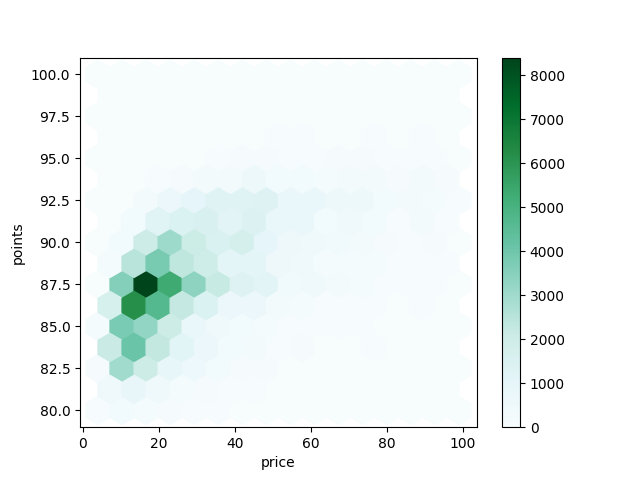
\includegraphics[width=0.8\textwidth]{hexbar}
		\caption{histogram cena i poena}
	\end{figure}
Takodje nam je interesantan atribut Variety. Prikazujemo 7 najcescih vrsta:
\begin{figure}[h!]
	\centering
		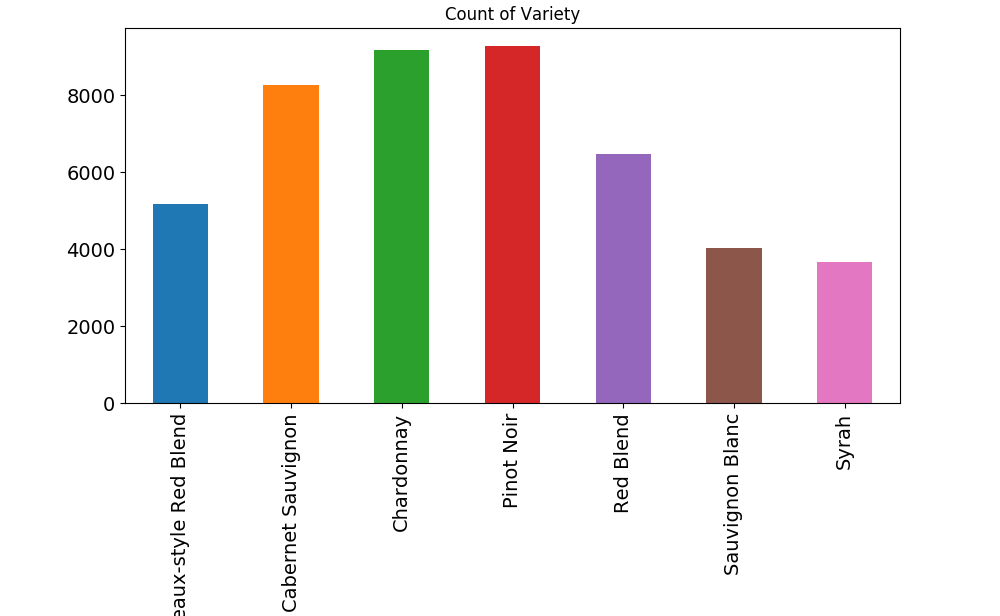
\includegraphics[width=0.8\textwidth]{variety_count}
	\end{figure}
	
	\newpage
	\section{Klasifikacija}
\subsection{Uvod}
Sa obzirom da nasi podaci predstavljaju recenzije, logicno je da se u analizi podataka fokusiramo upravo na tekstualne podatke.
Metode koje koristimo u nastavku spadaju u tzv NLTP odnosno natural language text processing, gde na osnovu pojedinacnih reci 
od kojih je sastavljen tekst recenzije pokusavamo da predvidimo vrednosti drugih atributa. Treba napomenuti da su ove radnje 
izuzetno memorijski zahtevne, te da je nemoguce raditi sa svim podacima. Samim tim dobijeni rezultati nisu toliko precizni,
ali bez obzira da li se radi o Python modulima ili cvoru u KNIME-u, nije moguce obraditi vise od 5\% podataka.
\subsection{Tag Cloud}
Pre nego sto pocnemo sa klasifikacijom, uradicemo interesantnu analizu koja proizvodi tzv. Tag Cloud, odnosno vizuelnu reprezentaciju 
teksta gde je vaznost reci reprezentovana pozicijom, velicinom i prozirnoscu. Dobijeni rezultat nam daje dobru ideju o tome koje reci su 
u najvecem fokusu u nasem istrazivanju.
\begin{figure}[h!]
	\centering
		\includegraphics[width=0.8\textwidth]{tag_cloud_print}
		\caption{KNIME workflow}
	\end{figure}
\begin{figure}[h!]
	\centering
		\includegraphics[width=0.8\textwidth]{tag_cloud_img}
	\end{figure}
	
	\newpage
\subsection{klasifikacija u KNIME-u}
Klasifikaciju vrsimo nad tekstualnim podacima atributa description. Cilj ove klasifikacije je da na osnovu teksta recenzije
procenimo o kojoj vrsti vina je rec, to jest koja je vrsdnost atributa variety. Klasifikacija je pokusana u programu KNIME uz pomoc
ekstenzije za obradu tekstualnih podataka 'Text Processing'.\newline
%objasnjenje razlicitih cvorova

%zasto nisu koriscene sve vrste
Prilikom klasifikovanja uz koriscenje svih vrsta vina dobijena je ogromna greska klasifikacije od oko 80\%, zato sto postoji cak 630
razlicitih vrsta, mnoge od kojih se pojavaljuju samo jendom ili dvaput, tako da prilikom uzorkovanja podataka prakticno je nemoguce 
odrediti vina ovih vrsta tacno klasifikovati. Zato cemo uzeti 7 najcescih vrsta, i opet pokrenuti program.\newline
Opet se javlja velika greska, tako da pokusavamo da klasifikujemo drzave iz kojih su vina. \newline
Proces klasifikacije mozemo podeliti u 3 faze:\newline Prvo ucitavamo podatke uz pomoc CSV Reader-a, zatim koriscenjem filtera izbacujemo
redove u kojima se pojavljuju null vrednosti. Onda uzmimamo nasumican uzorak od 2\% podataka za analizu, i izbacujemo vina koja kostaju vise od 
50 dolara.\newline U drugoj fazi koristimo cvorove iz Text Processing ekstenzije. Strings to Document cvor dodaje novu kolonu tipa Document.
Ovaj cvor nam je bitan jer u njemu mozemo da navedemo kategorije za redove koje cemo kasnije koristiti. Bag of Words Creator je cvor koji 
od svake reci pravi Term, odnosno razdvaja recenzije na reci. Sledecih nekoliko cvorova izbacuju interpunkcije, cesto koriscene reci i sl. Document
Vector cvor daje numericku vrednost svakom od Termova.\newline
Sada kada imamo numericke vrednosti mozemo da uradimo klasifikaciju. Category to Class cvor uzima kategorije koje smo naveli u ranijoj fazi i dodaje 
kolonu prema kojoj cemo vrsiti klasifikaciju. Koriscen je KNN klasifikator zato sto se najbrze izvrsava. Greska je oko 41\%.
\begin{figure}[h!]
	\centering
		\includegraphics[width=0.8\textwidth]{classification_print}
		\caption{histogram cena i poena}
	\end{figure}
\begin{figure}[h!]
	\centering
		\includegraphics[width=0.8\textwidth]{conf_matrix_print}
	\end{figure}
\newpage
\subsection{klasifikacija u jeziku Python}
Klasifikacija se izvrsava nad 10\% podataka, koji ukljucuju 10 vrsta vina koja se najcesce pojavljuju. Cilj ove klasifikacije je da 
na osnovu unetog teksta predvidimo koja je vrsta vina u pitanju. Prvo racunamo TFIDF (Term Frequency, Inverse Document Frequency)
 - numericku statistiku koje pokazuje koliko je bitna rec za odredjeni dokument. Ovu meru racunamo i za digrame, odnosno za parove reci.
\begin{lstlisting}
features = tfidf.fit_transform(df.Description).toarray()
labels = df.category_id
print(features.shape)

N = 2
for Variety, category_id in sorted(category_to_id.items()):
  features_chi2 = chi2(features, labels == category_id)
  indices = np.argsort(features_chi2[0])
  feature_names = np.array(tfidf.get_feature_names())[indices]
  unigrams = [v for v in feature_names if len(v.split(' ')) == 1]
  bigrams = [v for v in feature_names if len(v.split(' ')) == 2]
  print("# '{}':".format(Variety))
  print("  . Most correlated unigrams:\n. {}".format('\n. '.join(unigrams[-N:])))
  print("  . Most correlated bigrams:\n. {}".format('\n. '.join(bigrams[-N:])))
\end{lstlisting}
U konzoli ispisujemo najjbitnije reci i bigrame za svaku od vrsta vina:
\begin{lstlisting}
# 'Bordeaux-style Red Blend':
  . Most correlated unigrams:
. 92
. sample
  . Most correlated bigrams:
. 92 94
. barrel sample
# 'Cabernet Sauvignon':
  . Most correlated unigrams:
. cassis
. cab
  . Most correlated bigrams:
. flavors blackberries
. 100 cabernet
# 'Chardonnay':
  . Most correlated unigrams:
. chard
. chardonnay
  . Most correlated bigrams:
. tropical fruit
. buttered toast
# 'Merlot':
  . Most correlated unigrams:
. merlots
. merlot
  . Most correlated bigrams:
. chilean merlot
. 100 merlot
# 'Pinot Noir':
  . Most correlated unigrams:
. noir
. pinot
  . Most correlated bigrams:
. silky texture
. pinot noir
# 'Red Blend':
  . Most correlated unigrams:
. sangiovese
. blend
  . Most correlated bigrams:
. blend cabernet
. cabernet sauvignon
# 'Riesling':
  . Most correlated unigrams:
. lime
. riesling
  . Most correlated bigrams:
. yellow peach
. dry riesling
# 'Sauvignon Blanc':
  . Most correlated unigrams:
. gooseberry
. blanc
  . Most correlated bigrams:
. passion fruit
. sauvignon blanc
# 'Syrah':
  . Most correlated unigrams:
. syrahs
. syrah
  . Most correlated bigrams:
. rich syrah
. syrah offers
# 'Zinfandel':
  . Most correlated unigrams:
. zinfandel
. zin
  . Most correlated bigrams:
. briary brambly
. high alcohol
\end{lstlisting}
Vreme je da uradimo klasifikaciju. Koristimo naivni Bajesov klasifikator da treniramo nas model, koji zatim isprobavamo. Pritom za test koristimo 
bilo koji tekst, dakle ne moramo da koristimo vec postojecu recenziju. 
\begin{lstlisting}
X_train, X_test, y_train, y_test = train_test_split(df['Description'], df['Variety'], random_state = 0)
count_vect = CountVectorizer()
X_train_counts = count_vect.fit_transform(X_train)
tfidf_transformer = TfidfTransformer()
X_train_tfidf = tfidf_transformer.fit_transform(X_train_counts)

clf = MultinomialNB().fit(X_train_tfidf, y_train)

print(clf.predict(count_vect.transform(["Tannins and acidity"])))
#we get pinot noir as the prediction

print(clf.predict(count_vect.transform(["A rich blend of blackberry, strong flavors"])))
#we get red blend 
\end{lstlisting}
Uradicemo jos jednu klasifikaciju sa istim podacima koristeci SVM. Taj model testiramo 
sa test podacima i prikazujemo matricu konfuzije. Takodje u konzoli stampamo izvestaj.
\begin{lstlisting}
model = LinearSVC()

X_train, X_test, y_train, y_test, indices_train, indices_test = train_test_split(features, labels, df.index, test_size=0.33, random_state=0)
model.fit(X_train, y_train)
y_pred = model.predict(X_test)

conf_mat = confusion_matrix(y_test, y_pred)
fig, ax = plt.subplots(figsize=(10,10))
sns.heatmap(conf_mat, annot=True, fmt='d',
            xticklabels=category_id_df.Variety.values, yticklabels=category_id_df.Variety.values)
plt.ylabel('Actual')
plt.xlabel('Predicted')
plt.show() #prikazuje matricu konfuzije

print(metrics.classification_report(y_test, y_pred, target_names=df['Variety'].unique()))
\end{lstlisting}
\begin{figure}[h!]
	\centering
		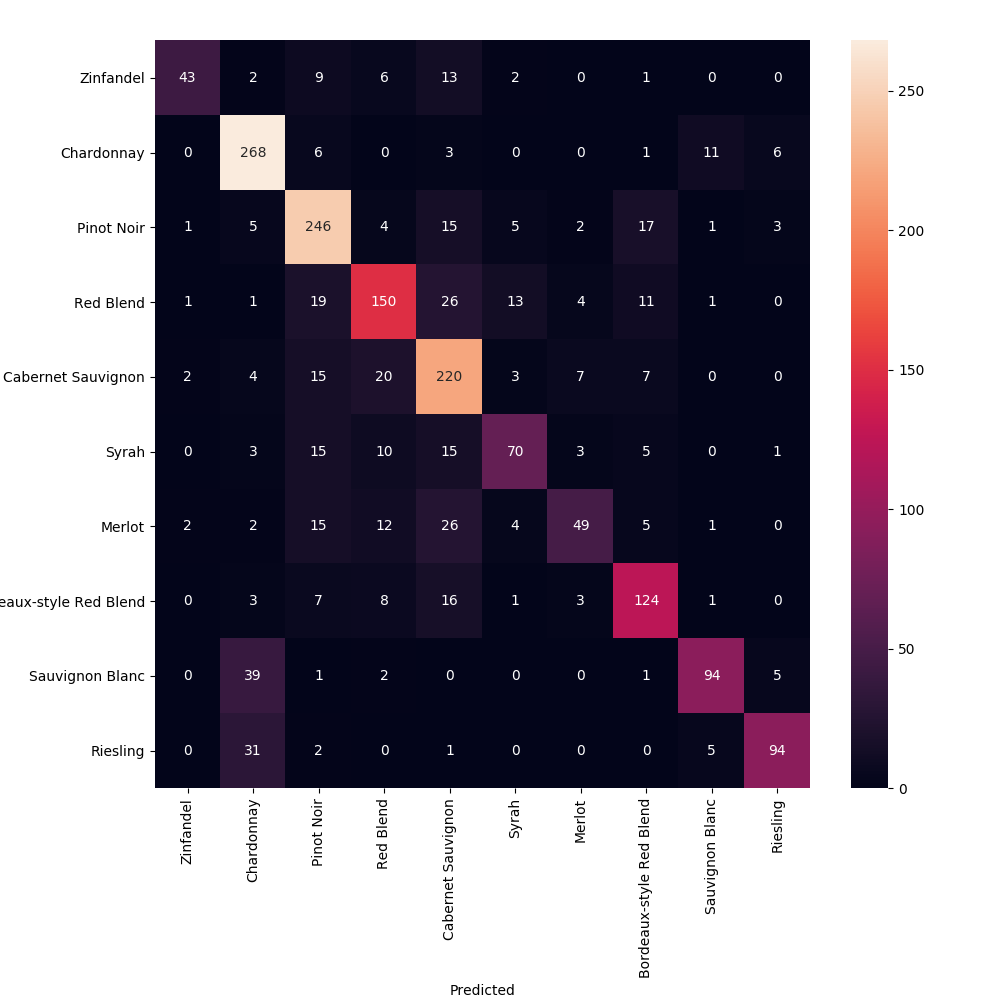
\includegraphics[width=0.8\textwidth]{conf_matrix_SVM}
		\caption{matrica konfuzije za SVM klasifikator}
	\end{figure}
\newpage
\begin{lstlisting}
                          precision    recall  f1-score   support

               Zinfandel       0.88      0.57      0.69        76
              Chardonnay       0.75      0.91      0.82       295
              Pinot Noir       0.73      0.82      0.78       299
               Red Blend       0.71      0.66      0.68       226
      Cabernet Sauvignon       0.66      0.79      0.72       278
                   Syrah       0.71      0.57      0.64       122
                  Merlot       0.72      0.42      0.53       116
Bordeaux-style Red Blend       0.72      0.76      0.74       163
         Sauvignon Blanc       0.82      0.66      0.73       142
                Riesling       0.86      0.71      0.78       133

             avg / total       0.74      0.73      0.73      1850
\end{lstlisting}
\newpage
\subsection{Analiza sentimenta}
Podelili smo podatke u dve kategorije - pozitivne i negativne kritike.Podela je izvrsena na osnovu poena koji su 
dodeljeni. Kako je raspon poena 80-100, podela je izvrsena na 90 poena. Cilj ove analize je da li mozemo da, na 
osnovu teksta recenzije, odredimo da li ce biti data pozitivna ili negativna ocena. Kod koji je koriscen je slican 
prethodnim primerima. Koristimo hi kvadrat metriku da odredimo znacaj reci na analizu sentimenta. Kada smo 
istrenirali model nad trening podacima, testiramo ga i stampamo rezultate. Takodje, crtamo graf koji prikazuje 
reci sa najvecom hi kvadrat vrednoscu - najbitnije reci za nasu analizu.
\begin{lstlisting}
import pandas as pd
from sklearn.feature_extraction.text import TfidfVectorizer
import numpy as np
from sklearn.model_selection import train_test_split
from sklearn.feature_extraction.text import CountVectorizer
from sklearn.metrics import accuracy_score
from sklearn.metrics import classification_report
from sklearn.feature_selection import chi2
import matplotlib.pyplot as plt

df = pd.read_csv('processed_data.csv')

tfidf = TfidfVectorizer()
tfidf.fit(df['description'])

X = tfidf.transform(df['description'])
\end{lstlisting}
\begin{lstlisting}
df.dropna(inplace=True)
df['Positivity'] = np.where(df['points'] > 90,1,0)
cols = ['country','designation','points','price','province', 'region_1','region_2', 'variety','winery']
df.drop(cols, axis=1, inplace=True)
df.head()

X = df.description
y = df.Positivity
X_train, X_test, y_train, y_test = train_test_split(X, y, random_state = 0)

print("Train set has total {0} entries with {1:.2f}% negative, {2:.2f}% positive".format(len(X_train),
 (len(X_train[y_train == 0]) / (len(X_train)*1.))*100, (len(X_train[y_train == 1]) / (len(X_train)*1.))*100))

print("Test set has total {0} entries with {1:.2f}% negative, {2:.2f}% positive".format(len(X_test),
 (len(X_test[y_test == 0]) / (len(X_test)*1.))*100, (len(X_test[y_test == 1]) / (len(X_test)*1.))*100))

cv = CountVectorizer()
rf = RandomForestClassifier(class_weight="balanced")

cv = CountVectorizer(max_features=10000,ngram_range=(1, 3))
pipeline = Pipeline([
        ('vectorizer', cv),
        ('classifier', rf)
    ])
sentiment_fit = pipeline.fit(X_train, y_train)
y_pred = sentiment_fit.predict(X_test)

print(classification_report(y_test, y_pred, target_names=['negative','positive']))

tfidf = TfidfVectorizer(max_features=10000,ngram_range=(1, 3))
X_tfidf = tfidf.fit_transform(df.description)
y = df.Positivity
chi2score = chi2(X_tfidf, y)[0]

plt.figure(figsize=(12,8))
scores = list(zip(tfidf.get_feature_names(), chi2score))
chi2 = sorted(scores, key=lambda x:x[1])
topchi2 = list(zip(*chi2[-20:]))
x = range(len(topchi2[1]))
labels = topchi2[0]
plt.barh(x,topchi2[1], align='center', alpha=0.5)
plt.plot(topchi2[1], x, '-o', markersize=5, alpha=0.8)
plt.yticks(x, labels)
plt.xlabel('$\chi^2$')
plt.show();
\end{lstlisting}
\begin{lstlisting}
Train set has total 19068 entries with 70.63% negative, 29.37% positive
Test set has total 6356 entries with 70.37% negative, 29.63% positive
             precision    recall  f1-score   support
 
   negative       0.78      0.92      0.85      4473
   positive       0.69      0.39      0.50      1883
 
avg / total       0.75      0.77      0.75      6356
\end{lstlisting}
\begin{figure}[h!]
	\centering
		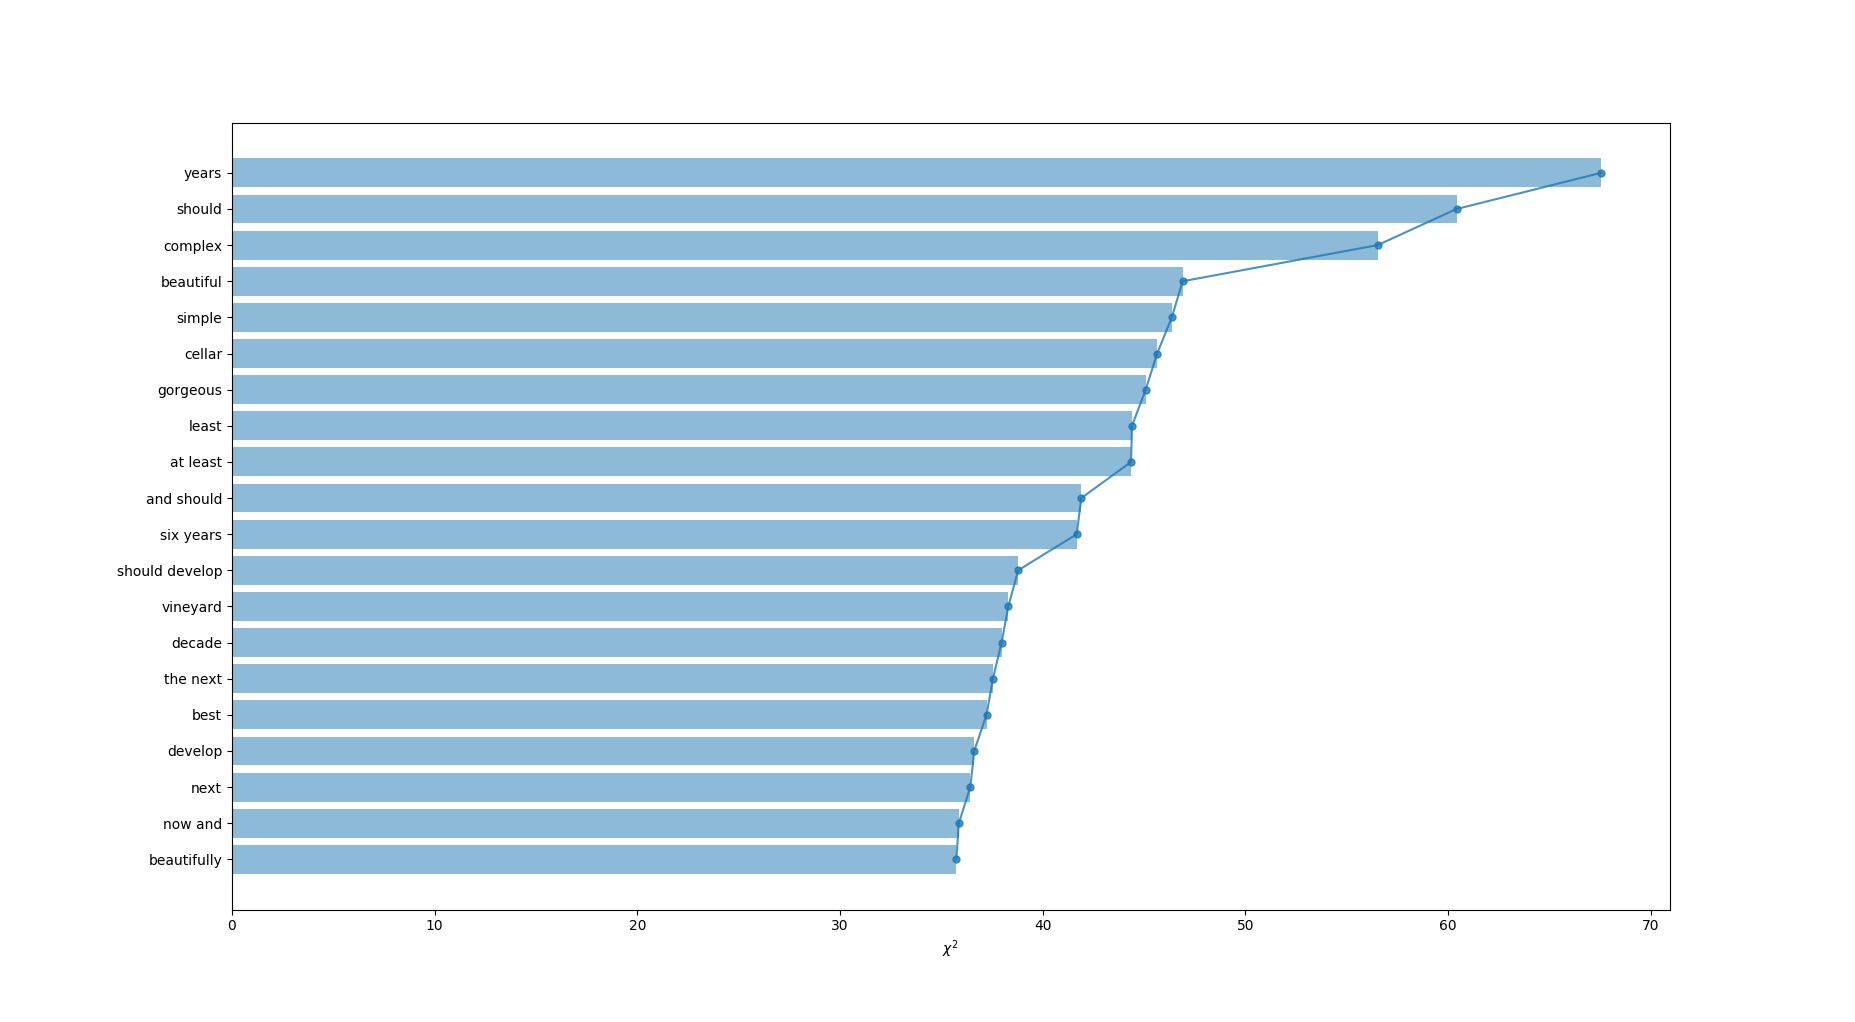
\includegraphics[width=1.4\textwidth]{chi_sentiment}
		\caption{hi kvadrat}
	\end{figure}
\newpage
\section{Klasterovanje}
\subsection{Klasterovanje u KNIME-u}
Proces klasterovanja lici na proces klasifikacije. U ovom primeru koristimo hijerarhijsko klasterovanje koje us pomoc 
matrice rastojanja grupise podatke. Medjutim, posto je broj nasih podataka jako velik, dobijeni dendogram je prilicno necitljiv.
\begin{figure}[h!]
	\centering
		\includegraphics[width=0.8\textwidth]{clustering_print}
		\caption{KNIME workflow}
	\end{figure}
\begin{figure}[h!]
	\centering
		\includegraphics[width=0.8\textwidth]{dendogram_clustering}
		\caption{matrica konfuzije za SVM klasifikator}
	\end{figure}

\subsection{Klasterovanje u Python-u}
Koristimo KMeans da formiramo 5 klastera reci koriscenih u tekstovima recenzija. Da bi prikazali rezultate, stampamo 10
najboljih reci po klasteru:

\begin{lstlisting}
from sklearn.feature_extraction.text import TfidfVectorizer
from sklearn.cluster import KMeans
from sklearn.metrics import adjusted_rand_score
import pandas as pd
import matplotlib.pyplot as plt 

df = pd.read_csv('processed_data.csv')
df = df.sample(frac=0.25)

documents = df['description']

vectorizer = TfidfVectorizer(stop_words='english')
X = vectorizer.fit_transform(documents)

true_k = 5
model = KMeans(n_clusters=true_k, init='k-means++', max_iter=100, n_init=1)
model.fit(X)

print("Top terms per cluster:")
order_centroids = model.cluster_centers_.argsort()[:, ::-1]
terms = vectorizer.get_feature_names()
for i in range(true_k):
    print("Cluster %d:" % i),
    for ind in order_centroids[i, :10]:
        print(' %s' % terms[ind]),
    print
\end{lstlisting}

\begin {lstlisting}
Top terms per cluster:
Cluster 0:  apple  flavors  citrus  peach  acidity  white  crisp  finish  wine  pear
Cluster 1:  flavors  dry  cherry  tannins  cherries  blackberry  oak  drink  wine  soft
Cluster 2:  aromas  black  cherry  palate  plum  berry  finish  flavors  fruit  red
Cluster 3:  wine  fruit  flavors  finish  cherry  aromas  notes  sweet  spice  oak
Cluster 4:  wine  fruits  acidity  tannins  ripe  wood  fruit  rich  character  aging
\end{lstlisting}
\newpage
\section{Pravila pridruzivanja}
Koristicemo KNIME da bismo pronasli pravila pridruzivanja. Najpre cemo izbaciti kolone region\_1 i 
region\_2 zato sto u vecini slucajeva one imaju iste ili veoma slicne vrednosti sa kolonom province, pa 
nam ta pravila nisu interesantna. Takodje izbacujemo kolonu description koja nam ne pomaze u ovoj analizi jer ta 
kolona ima sve jedinstvene vrednosti. Da bismo pokrenuli analizu moramo da spojimo kolone uz pomoc cvora 
Create Collection Column. Namestamo parametre u cvoru Association Rule Learner i stampamo tabelu.
\begin{figure}[h!]
	\centering
		\includegraphics[width=0.8\textwidth]{asc_rules_print}
		\caption{KNIME workflow}
	\end{figure}
\begin{figure}[h!]
	\centering
		\includegraphics[width=0.8\textwidth]{asc_rules_table}
		\caption{pravila pridruzivanja}
	\end{figure}

\end{document}



























